\chapter{Chuẩn bị}
    \section{RF Design}
        \subsection{Basics}
            \begin{itemize}
                \item Độ tự cm (L) được xác định bởi \textbf{hàm vòng lặp (Function of Loop)} của tín hiệu và đường phản hồi.
                Khoảng cách nhỏ (Tight loop) tạo ra khả năng triệt tiêu từ thông cao, do đó có độ tự cảm thấp.
                \item Điện dung (C) là \textbf{hàm khoảng cách (Function of Space)} của tín hiệu đến đường dẫn về. Khoảng cách nhỏ tạo ra điện dung cao.
                \item Vì Khoảng cách nhỏ (Tight loop) tạo ra L thấp và C cao và vì $Z_0 = \sqrt{\frac{L}{C}}$, nên Khoảng cách nhỏ tạo ra $Z_0$ thấp.
                \item Ngoài ra, $Z_0$ là hàm của Độ rộng và Độ dày của Dây dẫn tín hiệu và Hàm của Hằng số điện môi ($\epsilon_r$) của vật liệu xung quanh các đường dẫn.
                \item Bước sóng ($\lambda$) của tín hiệu là khoảng cách mà sóng truyền đi trong một chu kỳ sóng.
                \item Đối với tín hiệu truyền đi trong không gian tự do: $\lambda = \frac{c}{f}$
                \item Tín hiệu trong điện môi $\epsilon_r$ cao hơn: $\lambda = \frac{c}{f\sqrt{\epsilon_r}}$
                \item ??? Chiều dài tới hạn của đường truyền (Signal Critical Length): $L_{critical} = \frac{c}{16f\sqrt{\epsilon_r}}$.
            \end{itemize}

            \newpage
        \subsection{Transmission Line}
            \begin{longtable}{|m{0.15\textwidth} p{0.2\textwidth} p{0.65\textwidth}|}
                \hline
                \textbf{Model Parameter} & \textbf{Origin} & \textbf{Comment} \\\hline
                \endfirsthead
                \hline
                \textbf{Model Parameter} & \textbf{Origin} & \textbf{Comment} \\\hline
                \endhead
                \hline
                \endfoot
                \endlastfoot

                $R$ & Conductance & atomic property of metal used \\
                    & Geometry & larger cross section = lower $R$ \\
                    & & longer = higher $R$ \\
                    & Radiation & fields not contained are losses \\
                    & Skin Effect & current flows in smaller cross-section as frequency increases \\
                    & Proximity Effect & adjacent conductor's field forces current into smaller cross-section \\\hline

                $L$ & Permeability & property of metal used \\
                    & Geometry & larger cross section = lower $L$ \\
                    & & longer = higher $L$ \\
                    & Skin Effect & currents at different depths in conductor have different phases, net effect is inductive \\
                    & Proximity & adjacent conductor's field forces current into smaller cross-section \\
                    & Radiation & \\\hline

                $C$ & Geometry & larger area = higher $C$ \\
                    & & closer conductors = higher $C$ \\
                    & Permittivity & higher $\epsilon_r$ = higher $C$ \\\hline

                $G$ & Loss Tangent & higher loss tan = higher losses in dielectric \\
                    & Conductance & semiconductor dielectrics \\
                    & Geometry & \\\hline
                
                \caption{Transmission Line Model Parameters and Sources}
            \end{longtable}
            




    \section{Bluetooth Low Energy (BLE) Module}
        \subsection{Thông tin IC}
        \subsection{Thiết kế}
            \subsubsection{IC recommendations}
                \paragraph{Power}
                \paragraph{XTAL, 32 MHz (Y1)}
                    \begin{longtable}{|m{0.2\textwidth}|m{0.15\textwidth}|m{0.25\textwidth}|>{\centering\arraybackslash}m{0.075\textwidth}|>{\centering\arraybackslash}m{0.075\textwidth}|>{\centering\arraybackslash}m{0.075\textwidth}|>{\centering\arraybackslash}m{0.075\textwidth}|}
                        \hline
                        \textbf{Symbol} & \textbf{Parameter} & \textbf{Conditions} & \textbf{Min.} & \textbf{Typ.} & \textbf{Max.} & \textbf{Unit} \\\hline
                        \endfirsthead
                        \hline
                        \textbf{Symbol} & \textbf{Parameter} & \textbf{Conditions} & \textbf{Min.} & \textbf{Typ.} & \textbf{Max.} & \textbf{Unit} \\\hline
                        \endhead
                        \hline
                        \endfoot
                        \endlastfoot
                        
                        fXTAL\_32M & crystal oscillator frequency & & & 32 & & MHz \\\hline
                        $\Delta$fXTAL & crystal frequency tolerance & After optional trimming; including aging and temperature drift. & -20 & & 20 & ppm \\\hline
                        $\Delta$fXTAL\_UNT & crystal frequency tolerance & Untrimmed; including aging and temperature drift. & -40 & & 40 & ppm \\\hline
                        ESR\_1 & equivalent series resistance & C0=3pF & & & 100 & $\Omega$ \\\hline
                        ESR\_2 & equivalent series resistance & C0=5pF & & & 60 & $\Omega$ \\\hline
                        C0\_1 & shunt capacitance & ESR=100$\Omega$ & & & 3 & pF \\\hline
                        C0\_2 & shunt capacitance & ESR=60$\Omega$ & & & 5 & pF \\\hline
                        CL & load capacitance & No external capacitors are required & 4 & 6 & 8 & pF \\\hline
                        
                        \caption{XTAL32 MHz Oscillator - Recommended Operating Conditions}
                    \end{longtable}
                
                \paragraph{XTAL, 32.768 kHz (Y2)}
                    \begin{longtable}{|m{0.2\textwidth}|m{0.15\textwidth}|m{0.25\textwidth}|>{\centering\arraybackslash}m{0.075\textwidth}|>{\centering\arraybackslash}m{0.075\textwidth}|>{\centering\arraybackslash}m{0.075\textwidth}|>{\centering\arraybackslash}m{0.075\textwidth}|}
                        \hline
                        \textbf{Symbol} & \textbf{Parameter} & \textbf{Conditions} & \textbf{Min.} & \textbf{Typ.} & \textbf{Max.} & \textbf{Unit} \\\hline
                        \endfirsthead
                        \hline
                        \textbf{Symbol} & \textbf{Parameter} & \textbf{Conditions} & \textbf{Min.} & \textbf{Typ.} & \textbf{Max.} & \textbf{Unit} \\\hline
                        \endhead
                        \hline
                        \endfoot
                        \endlastfoot
                        
                        fXTAL\_32M & crystal oscillator frequency & & 30 & 32.768 & 35 & kHz \\\hline
                        ESR & equivalent series resistance & & & & 100 & k$\Omega$ \\\hline
                        CL & load capacitance & No external capacitors are required for a 6pF or 7pF crystal & 6 & 7 & 9 & pF \\\hline
                        C0 & shunt capacitance & & & 1 & 2 & pF \\\hline
                        PDRV\_MAX & maximum drive power & & 0.1 & & & $\mu$W \\\hline
                        $\Delta$fXTAL & crystal frequency tolerance (including aging) & Timing accuracy is dominated by crystal accuracy. A much smaller value is dominated & -250 & & 250 & ppm \\\hline
                        
                        \caption{XTAL Oscillator 32kHz - Recommended Operating Conditions}
                    \end{longtable}

                \paragraph{Reset}
                \paragraph{JTAG}
                \paragraph{UART}
                \paragraph{SPI Data Flash}
                \paragraph{RF}
                    \begin{itemize}
                        \item DA14531 provides a 50 Ohms single RFIO port for Tx and Rx without requiring external balun or RF switch. The internal RF power amplifier provides Tx RF power from -19.5 dBm to +2.5 dBm.
                        \item Working in 2.4 GHz  Bluetooth low energy.
                    \end{itemize}
            
            \subsubsection{Sơ đồ tổng quát}
                \begin{figure}[h]
                    \centering
                    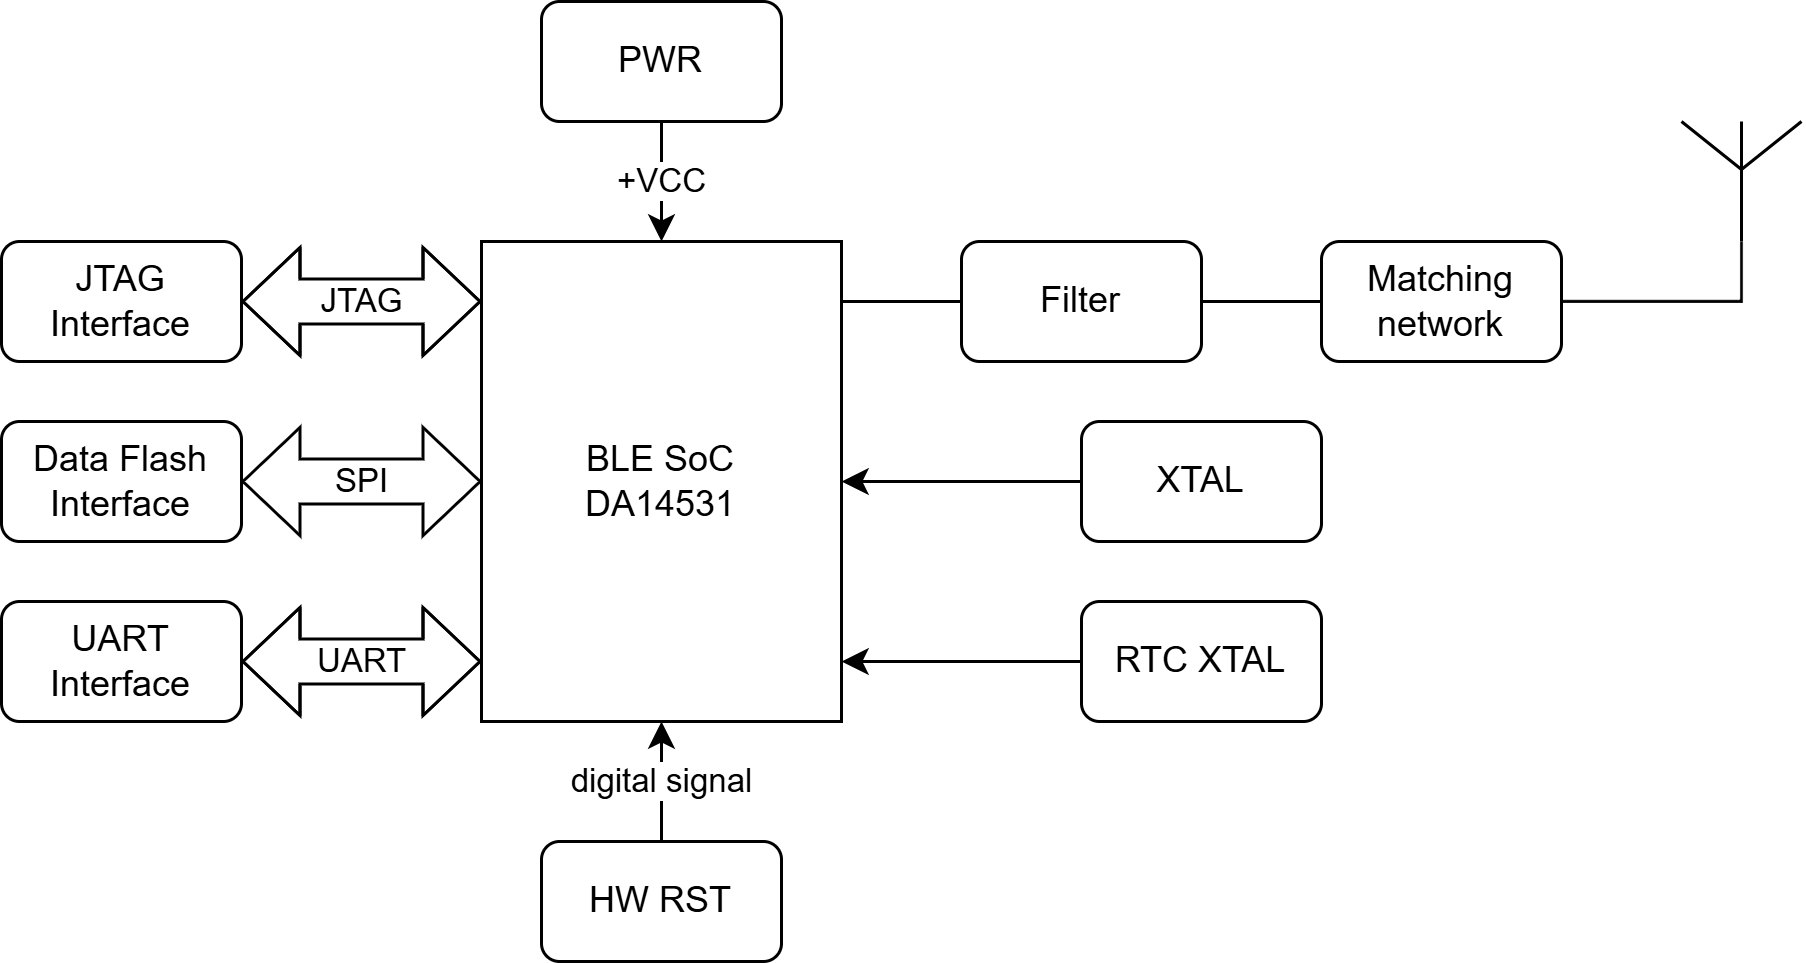
\includegraphics[width=0.8\textwidth]{figures/DA14531_diagram.drawio.png}
                    \caption{Sơ đồ tổng quát}
                \end{figure}

            \subsubsection{Transmission line}
                \begin{figure}[h]
                    \centering
                    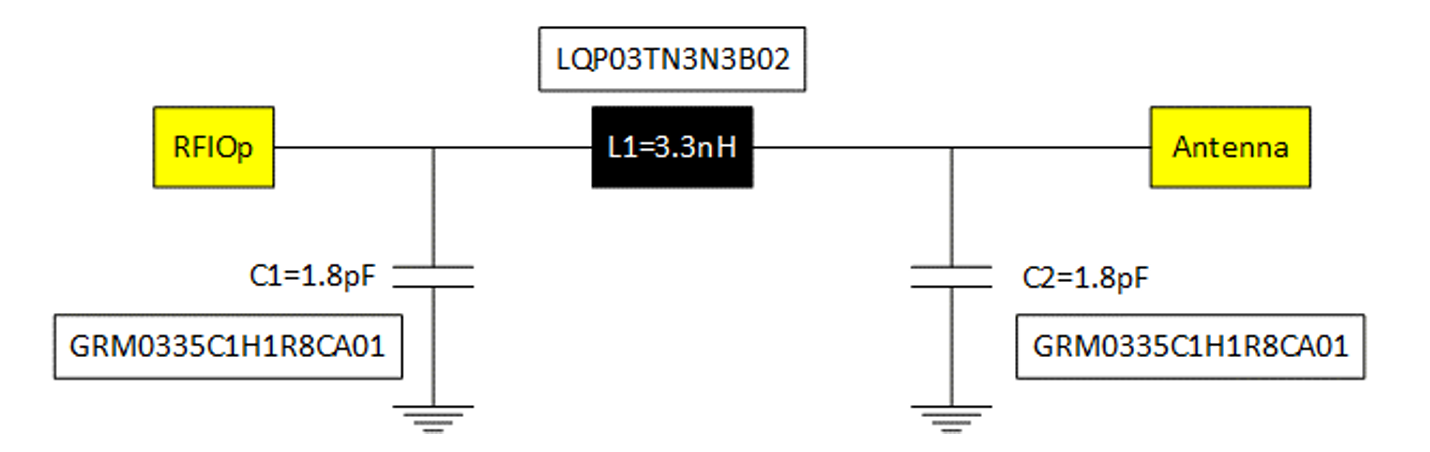
\includegraphics[width=0.8\textwidth]{figures/pi_filter.png}
                    \caption{Pi Filter Topology}
                \end{figure}
                Calculation tool: \url{https://www.electronics-tutorials.ws/tools/pi-pad-impedance-calculator.html}\par
                
                % Mạch Pi Filter sử dụng như mạch lọc, đồng thời có thể dùng để impedance matching.\par
                Equation:
                \begin{equation}
                    f_c = \frac{1}{2\pi\sqrt{LC_{eqv}}}
                \end{equation}

                \begin{equation}
                    C_{eqv} = \frac{C_1C_2}{C_1 + C_2}
                \end{equation}

                \begin{equation}
                    Q = \frac{f_0}{BW} = \frac{f_0}{\Delta f}
                \end{equation}

                \begin{equation}
                    X_{C_1} = \frac{Z_S}{Q}
                \end{equation}

                \begin{equation}
                    X_{C_2} = \frac{Z_{ant}}{\sqrt{\frac{Z_{ant}}{Z_S}\left(1+Q^2\right) - 1}}
                \end{equation}

                \begin{equation}
                    X_L = \frac{QR}{1+Q^2}\left[1 + \frac{1}{Q}\sqrt{\frac{Z_{ant}}{Z_S}\left(1+Q^2\right)-1}\right]
                \end{equation}

                \begin{equation}
                    Z_{input} = \left\{\left[Z_{ant} // Z_{C_2}\right] + Z_L\right\} // Z_{C_1}
                \end{equation}

                
                \begin{equation}
                    Z_{input} = \left\{\left[\left(R_{ant}+jX_{ant}\right) // \left(\frac{1}{j\omega C_2}\right)\right] + j\omega L\right\} // \left(\frac{1}{j\omega C_1}\right)
                \end{equation}

                \begin{equation}
                    Z_{input} = \left\{\left\{\left[\left(R_{ant}+jX_{ant}\right)^{-1} + \left(\frac{1}{j\omega C_2}\right)^{-1}\right]^{-1} + j\omega L\right\}^{-1} + \left(\frac{1}{j\omega C_1}\right)^{-1}\right\}^{-1}
                \end{equation}
            \subsubsection{Antenna}
